\section{Software architecture}

\begin{figure}
  \centering
  \makebox[\textwidth][c]{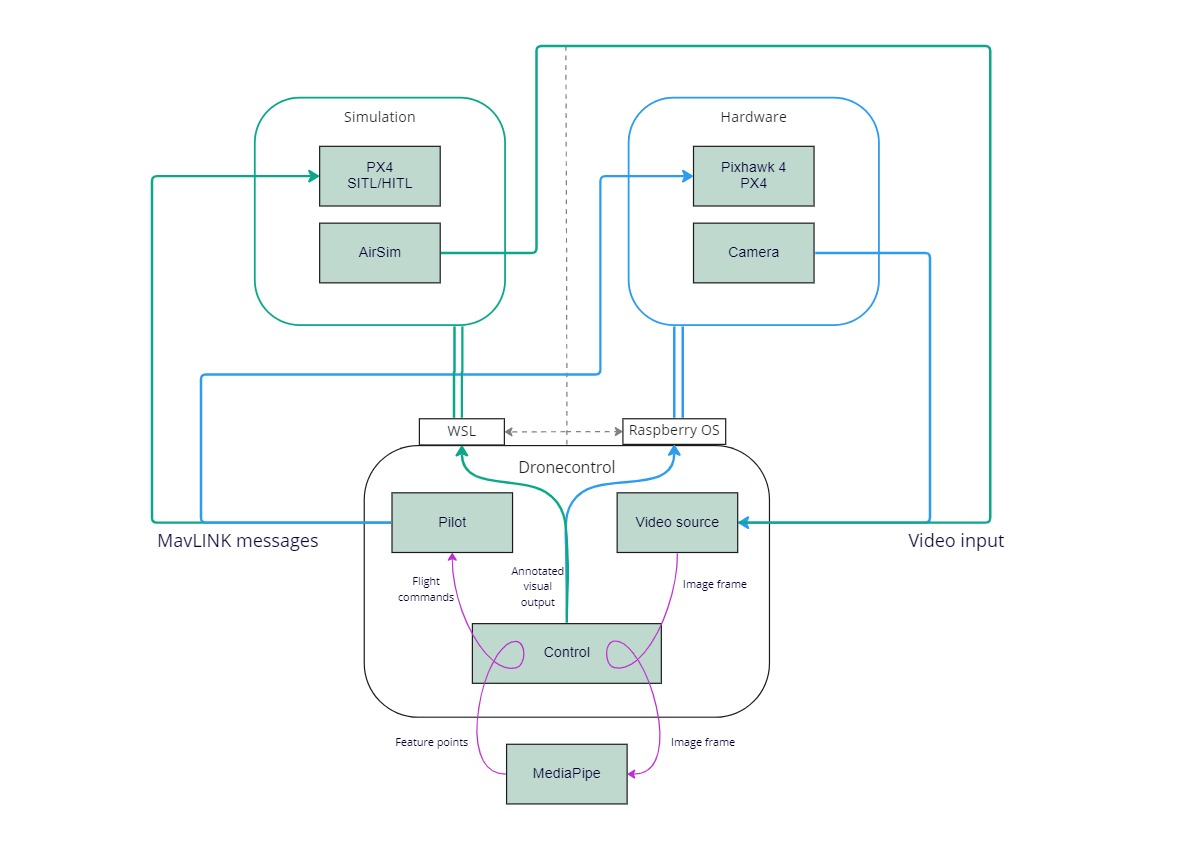
\includegraphics[width=1.2\textwidth, keepaspectratio]{img/software-arch.jpg}}
  \caption{Structure of the Dronecontrol application and its interactions with the necessary additional software for running in a simulation (green) or a vehicle (blue).}
\label{fig:architecture}
\end{figure}


Figure \ref{fig:architecture} shows the main modules of the designed software and how it interacts with the external libraries.
The application consists of three fundamental parts: the \textbf{pilot module}, in charge of sending instructions to the flight controller and receiving back information on position and state through the \texttt{mavsdk} library, 
a \textbf{video source module} that handles the retrieval of images from different sources and the necessary processing for image analysis,
and a \textbf{control module} that directs the interaction between the other two to transform the pixel information first into position points through the \texttt{mediapipe} library and then into instructions for the pilot.
The upper part of the diagram in figure \ref{fig:architecture} shows the flow of information between the Dronecontrol application and the external systems, with green lines representing its path in a simulated workflow and blue ones indicating the alternative path for the information in a system with actual quadcopter hardware.
Purple arrows show the input/output of each module within the developed application and how they interconnect.
Other smaller utilities have also been developed to help test how the systems interact with each other and calibrate different parts of the control behaviour.
These are described in sections \ref{subsec:cam-tool} and \ref{subsec:pid-tools}.
A user manual with all the options available in the application can be found in Appendix \ref{app:cli}.

\subsection{Pilot module}
\label{subsec:pilot-module}
The purpose of the pilot module\footnote{\url{https://github.com/l-gonz/tfg-giaa-dronecontrol/blob/main/dronecontrol/common/pilot.py}} is to provide access to the rest of the application to send and receive messages from the PX4 controller through the MavSDK library.
This library provides a simple asynchronous API for managing one or more vehicles, providing programmatic access to vehicle information and telemetry, and control over missions, movement and other operations.
MavSDK utilizes the Python library \texttt{asyncio} to run coroutines in parallel while waiting for the messages provided through the MAVLink communication.
Therefore all calls to the library have to be written as async functions that await the result of one or more polls to the flight stack.

\texttt{asyncio} provides support for writing concurrent code using the \texttt{async/await} syntax.
It is used as a foundation for multiple Python asynchronous frameworks that provide high-performance network and web servers, database connection libraries or distributed task queues.
It provides a set of high-level APIs to run Python coroutines concurrently and have complete control over their execution.
The pilot module integrates \texttt{mavsdk} and \texttt{asyncio} and provides a queue for the control module to send actions to be executed in the vehicle one after another.

Listing \ref{lst:pilot-connect} shows how to establish a connection to a PX4 vehicle through its physical serial address or virtual UDP one and poll for internal information from the flight controller to decide when the system is ready to receive instructions.
The MAVSDK library exposes telemetry and other state information through asynchronous generators, which are defined in python as a convenient way to make asynchronous data producers and accessed with the \texttt{async\ for} syntax.


\begin{listing}[h]
    \caption{Example of how the communication to the flight stack is established through \texttt{asyncio} and the MAVSDK library}{}
    \label{lst:pilot-connect}
    \begin{minted}[breaklines, fontsize=\footnotesize, baselinestretch=1]{python}
async def connect(self):
    """Connect to mavsdk server.
       Raises a TimeoutError if it is not possible to establish connection.
    """
    
    if self.serial:
        address = f"serial://{self.serial}"
    else:
        address = f"udp://{self.ip if self.ip else ''}:{self.port}"
    self.log.info("Waiting for drone to connect on address " + address)
    await asyncio.wait_for(self.mav.connect(system_address=address), timeout=self.TIMEOUT)

    async for state in self.mav.core.connection_state():
        if state.is_connected:
            break

    # Wait for drone to have a global position estimate
    async for health in self.mav.telemetry.health():
        if health.is_global_position_ok:
            break
        
    self.log.info("System ready")
    self.is_ready = True
    \end{minted}
\end{listing}

Many of the basic operations that can be executed in the flight controller are implemented in the pilot module, along with error handling and safety checks, like takeoff, landing, return home or manipulating the vehicle flying velocity directly by providing speeds in body coordinates.
These actions can be executed directly or added to a queue that is polled periodically to run them in the order that they are added, waiting until the previous action has finished and the vehicle is in the desired state before starting the next.
The loop that runs this queue can be seen in listing \ref{lst:pilot-queue}.
There is a maximum time of 10 seconds that each action can use to run.
The loop stops when the asynchronous task it runs on is cancelled with \mintinline{python}{task.cancel()}, which raises a \mintinline{python}{CancelledError} exception in the execution thread.

\begin{listing}[h]
    \caption{Loop where the action queue runs on the pilot module. Each action is awaited until it finishes or the timeout time runs out.}{}
    \label{lst:pilot-queue}
    \begin{minted}[breaklines, fontsize=\footnotesize, baselinestretch=1]{python}
async def run_queue(self):
    """
    Run the queue loop.
    
    Queued actions will be awaited one at a time
    until they are finished.
    The loop will sleep if the queue is empty.
    """
    try:
        while True:
            if len(self.actions) > 0:
                action = self.actions.pop(0)
                self.log.info("Execute action: %s", action.func.__name__)
                try:
                    await asyncio.wait_for(action.func(self, **action.args), timeout=10)
                except asyncio.exceptions.TimeoutError:
                    self.log.warning(f"Time out waiting for {action.func.__name__}")
            else:
                await asyncio.sleep(self.WAIT_TIME)
    except asyncio.exceptions.CancelledError:
        self.log.warning("System stop")
    \end{minted}
\end{listing}

\todo[inline]{Polish: consider removing code or exchanging for diagrams}

\subsection{Video source module}
\label{subsec:viz-source-module}

The objective of the \texttt{video\_source} module\footnote{\url{https://github.com/l-gonz/tfg-giaa-dronecontrol/blob/main/dronecontrol/common/video_source.py}} is to provide a collection of classes to retrieve images from different sources,
in a way that they can be exchanged for one another without affecting the rest of the application to facilitate testing and be adaptable to running in different environments.
Three classes of video sources have been implemented: file, simulator, and camera, which inherit from the same \texttt{VideoSource} according to the diagram in figure \ref{fig:video-source-inheritance}.

\begin{figure}
  \centering
  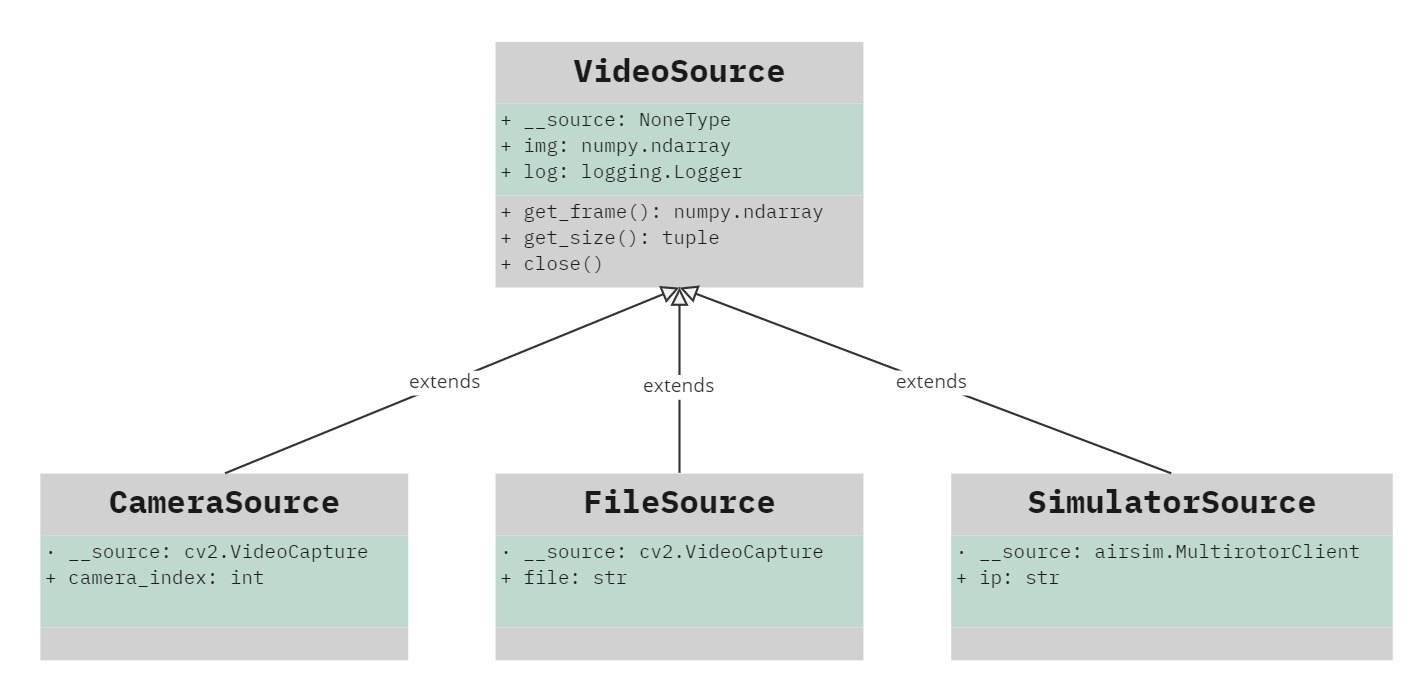
\includegraphics[width=\textwidth, keepaspectratio]{img/uml-video-source.jpg}
  \caption{Diagram of inheritance on the video source classes available to retrieve image data.}
  \label{fig:video-source-inheritance}
\end{figure}

The \texttt{FileSource} class is able to open a video file stored in the companion computer and provide images taken frame by frame from it until the video completes.
This allows the program to replay the image detection algorithms on videos previously captured by the camera tool described in section \ref{subsec:cam-tool}.
The \texttt{CameraSource} class can access a physical camera attached to the computer running the application via USB and provide the captured frames in real time.
Both the file and camera sources make use of OpenCV's video capture utilities to take care of the file handling and the camera drivers necessary.

The \texttt{SimulatorSource} uses AirSim's Python library \texttt{airlib} to communicate with the simulator and retrieve images from a camera object attached to the model of the vehicle in Unreal Engine.
It connects automatically through \texttt{localhost}, but it can also be initialized with an IP to establish a connection to the simulator running on a different computer on the local network; for example, when the Dronecontrol runs inside WSL and the simulator runs on the host computer.

\subsection{Vision control module}
\label{subsec:control-module}
The control module contains the main logic of the application and is in charge of converting the raw images obtained from the video source into commands for the pilot module.
Two different types of control have been implemented.
The first one is the proof-of-concept control solution described in section \ref{sec:hands} that operates in the offboard configuration outlined in section \ref{subsec:offboard} and translates predefined hand gestures into commands for the aerial vehicle.
The primary purpose is to be able to test the interaction between all the system components in an easily controlled environment thanks to using the more straightforward configuration of situating the controlling computer outside of the vehicle.
The second control system consists of a follow solution which attempts to reproduce an environment closer to real-life scenarios, where the control algorithms and the camera are onboard the vehicle.
It functions by tracking the location of a person detected in the images obtained from the drone's perspective, which is used to calculate the velocities required to follow said person and maintain it centred in its view.

The process followed in both solutions consists roughly of the same two parts.
First, the image is sent to the computer vision and machine learning third-party library (MediaPipe) that extracts the required features from the image in the form of 2D coordinates.
Afterwards, various calculations depending on the particular solution are applied to these coordinates to decide which commands are sent to the pilot module.
The third-party library used for computer vision in the program is the MediaPipe library described in section \ref{subsec:mediapipe}, which offers cross-platform, customizable machine-learning solutions appropriate for live and streaming media.

To engage the module in direct control of the vehicle's velocity, it is necessary to use a special flight mode defined by PX4 for this purpose, called Offboard mode\footnote{\url{https://docs.px4.io/main/en/flight_modes/offboard.html\#offboard-mode}} (not to be confused with the offboard configuration described in section \ref{subsec:offboard}).
Offboard mode primarily controls vehicle movement and attitude and supports only a minimal set of MAVLink messages.
This mode requires position or pose/attitude information to be available to the flight controller, for example, through a GPS antenna.
In it, the vehicle obeys a position, velocity or attitude setpoint provided over MAVLink by a MAVLink API (i.e. MAVSDK) running on a companion computer and usually connected via serial cable or wifi.
The vehicle must receive a stream of setpoint commands at a rate higher than 2Hz before engaging the mode to remain in it.
If the message rate falls below 2Hz or the connection is lost, the vehicle will stop and, after a timeout, attempt to land or perform some other failsafe action according to the parameters configured.

Sections \ref{sec:hands} and \ref{sec:follow} further explain the control modules used by the two different solutions developed.

\subsubsection{Camera-testing tool}
\label{subsec:cam-tool}

In addition to the main modules, several utilities have been added to the Dronecontrol program to facilitate the development and testing process of the control solutions.
The first tool is found on the \texttt{test\_camera} module\footnote{\url{https://github.com/l-gonz/tfg-giaa-dronecontrol/blob/main/dronecontrol/tools/test_camera.py}} and accessed through the command \texttt{dronecontrol tools test-camera}.
It can be used to test the connection between the computer, the flight stack and the camera without using any self-guided control mechanism, as well as to evaluate the performance of the MediaPipe hand and pose machine learning solution on real-time images.
It is also possible to capture images and record video from the live camera feed for later analysis.
Through the command-line options, the test tool can be configured to use any of the three available video sources: camera, simulator or any video file; to connect to an optional hardware or simulated PX4 flight controller by specifying a connection string or IP, respectively,
to run either in a host computer or a WSL subsystem;
Additionally, computer vision can be enabled to process incoming images through the hand or pose recognition software.
While the tool is running, the keyboard can be used to send basic commands to a connected vehicle like takeoff, landing or moving along any of its three axes.
A full breakdown of all the tool's options can be found in appendix \ref{app:cli}.


\section{Proof of concept: hand-gesture solution}
\label{sec:hands}
The main purpose of this solution is to test that the flow of the application works as expected, both in simulation and in actual flight, and that all the systems can interact and establish the required connections with each other.
For that reason, it is designed to run in flight with the minimal setup of a PX4-driven drone with its default components and any computer with a camera.

\begin{figure}
  \centering
  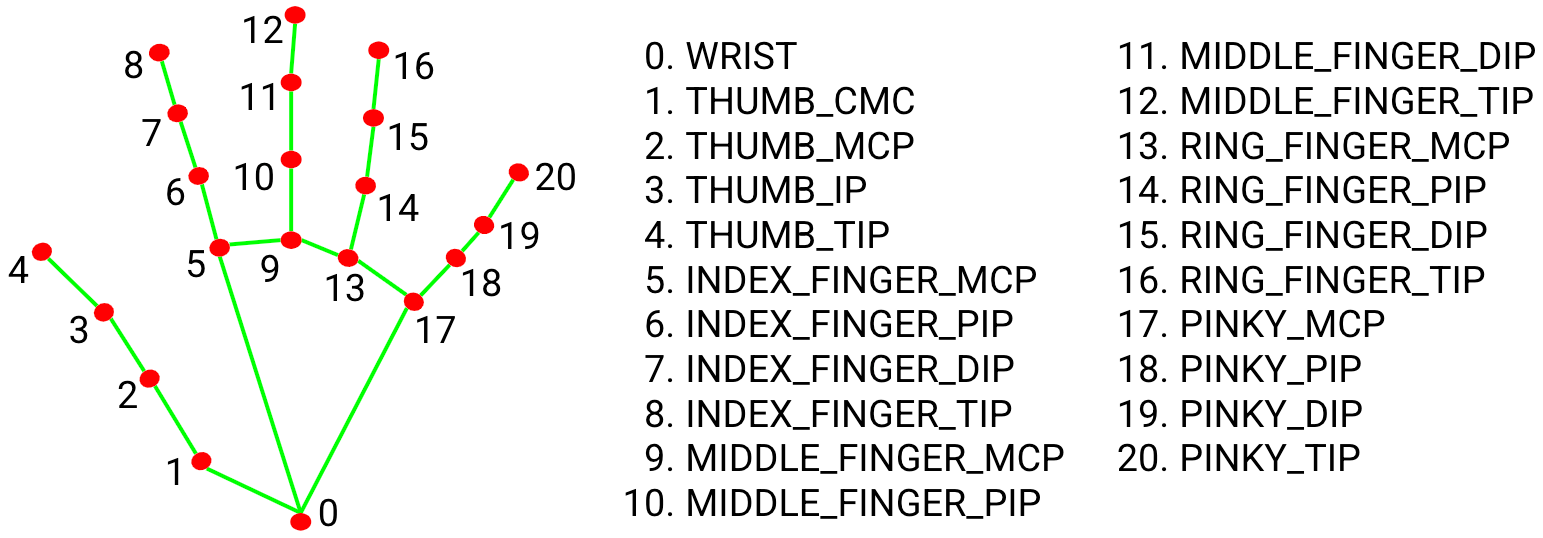
\includegraphics[width=\textwidth, keepaspectratio]{img/hand_landmarks.png}
  \caption{Landmarks extracted from detected hands by the MediaPipe hand solution.}
  \source{Adapted from \citetitle{mp-hands} \cite{mp-hands}.}
  \label{fig:hand-landmarks}
\end{figure}

This control module for this solution is the \texttt{mapper} module\footnote{\url{https://github.com/l-gonz/tfg-giaa-dronecontrol/blob/main/dronecontrol/hands/mapper.py}}.
It runs on a loop that continuously polls for a new frame from the chosen video source and feeds it to the hand detection functionality from MediaPipe \cite{mp-hands-paper}.
If a hand is detected in the images, 2D coordinates are extracted according to the map in figure \ref{fig:hand-landmarks}.
These landmarks are then converted into discrete gestures like an open palm, closed fist or a specific finger pointing in different directions.
When a new gesture is detected, the command assigned to it is queued to the pilot module and executed as soon as the previous commands end their execution.

The conversion between landmarks and gestures is performed by the \texttt{gestures} module\footnote{\url{https://github.com/l-gonz/tfg-giaa-dronecontrol/blob/main/dronecontrol/hands/gestures.py}}, drawing vectors from the base of each of the fingers to their tips as well as from the base of the hand (wrist feature) to the base of the fingers and using the dot product vector operation to calculate the relative angles between each finger and the base of the hand, as shown in figure \ref{fig:vector-calcs}.
By comparing the calculated angles to a threshold, it is possible to detect whether each individual finger is extended or folded, as well as the general direction toward which it points.
The open hand gesture, for example, can then be defined as all five fingers extended, that is, all five vectors defined by the fingers sharing the same approximate angle with the vector from the base of the hand to that finger.

\begin{figure}
  \centering
  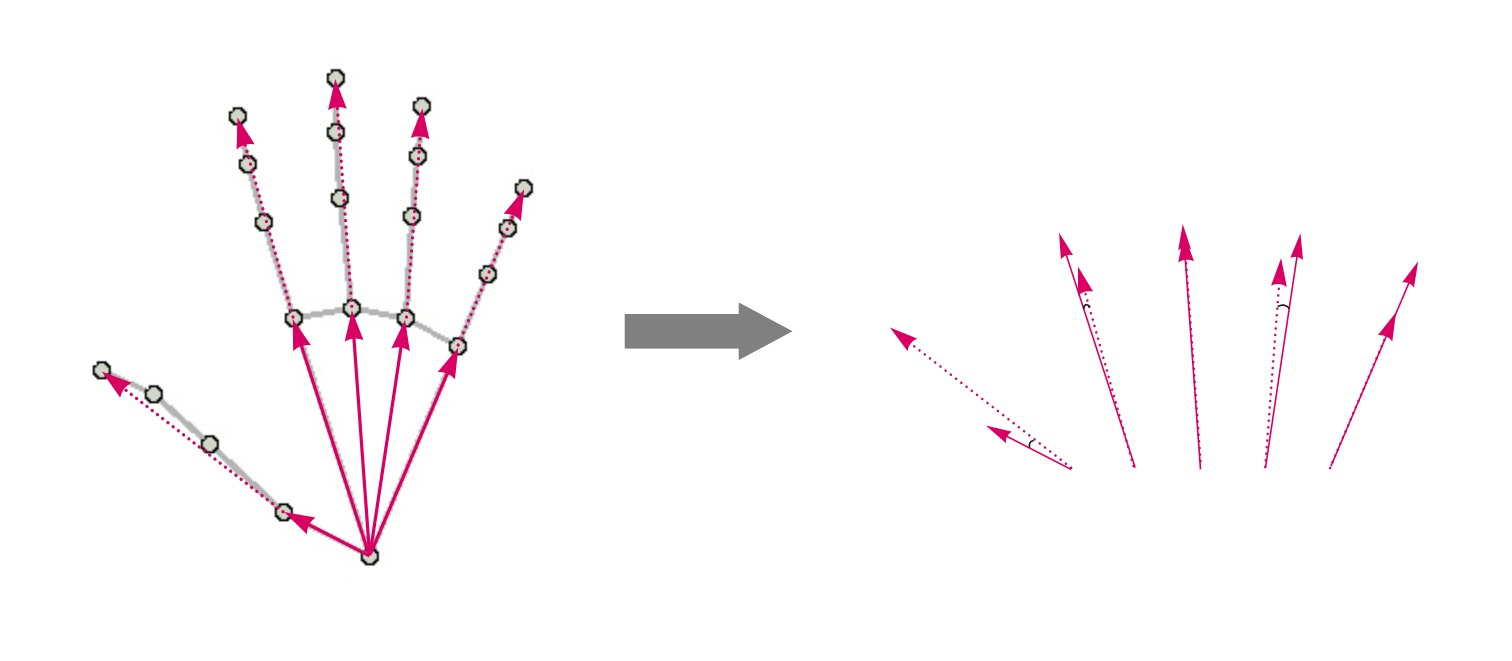
\includegraphics[width=0.9\textwidth, keepaspectratio]{img/hand-vectors.jpg}
  \caption{Vectors extracted from the detected features to calculate the angles between them and determine their relative positions.}
  \label{fig:vector-calcs}
\end{figure}

The full list of gestures detected by the program by calculating these angles is shown in figure \ref{fig:hand-gestures} and is as follows:
\begin{itemize}
    \item No hand: this happens when no landmarks can be extracted from the image. As a safety feature, the vehicle stops whichever previous commands it had in its queue and goes into "hold" flight mode, hovering in the air while maintaining its position.
    \item Open hand: it is detected when all five fingers are extended, as if gesturing stop. In this case, it makes the drone purposefully hold at its current position.
    \item Fist: it is detected when all five fingers are folded, forming a fist. It makes the drone arm and take off if it is on the ground or land if it is already in the air.
    \item Backhand: it is detected when the back of the hand is shown towards the camera, with the thumb pointing upwards and the other fingers pointing to the side, and makes the drone go into "return" flight mode, where it climbs to a configured, safe altitude and returns to the last takeoff position.
    \item Index finger pointing up: it is detected when the index finger is extended and pointing roughly towards the top of the image ($\pm 30$ degrees). It makes the drone go into "offboard" mode, where it is possible to receive direct velocity commands. The drone will remain in this mode while this finger is kept extended, and its movement can be controlled by adding one of the following four commands.
    \item Index finger pointing to the right: same as above but pointing to the right of the image, between 30 and 90 degrees from the top. It makes the drone roll towards its right side at a speed of 1 m/s.
    \item Index finger pointing to the left: same as above, but as the finger points to the left, so does the drone roll towards its left side.
    \item Thumb pointing to the right: it is detected when the index finger is extended up (to maintain the drone in offboard mode) and the thumb is folded, pointing towards the right of the screen. This gesture makes the drone pitch forward at a steady speed of 1 m/s.
    \item Thumb pointing to the left: same as the previous gesture, but the drone pitches backwards when the thumb points to the left of the screen.
\end{itemize}

\begin{figure}
  \centering
  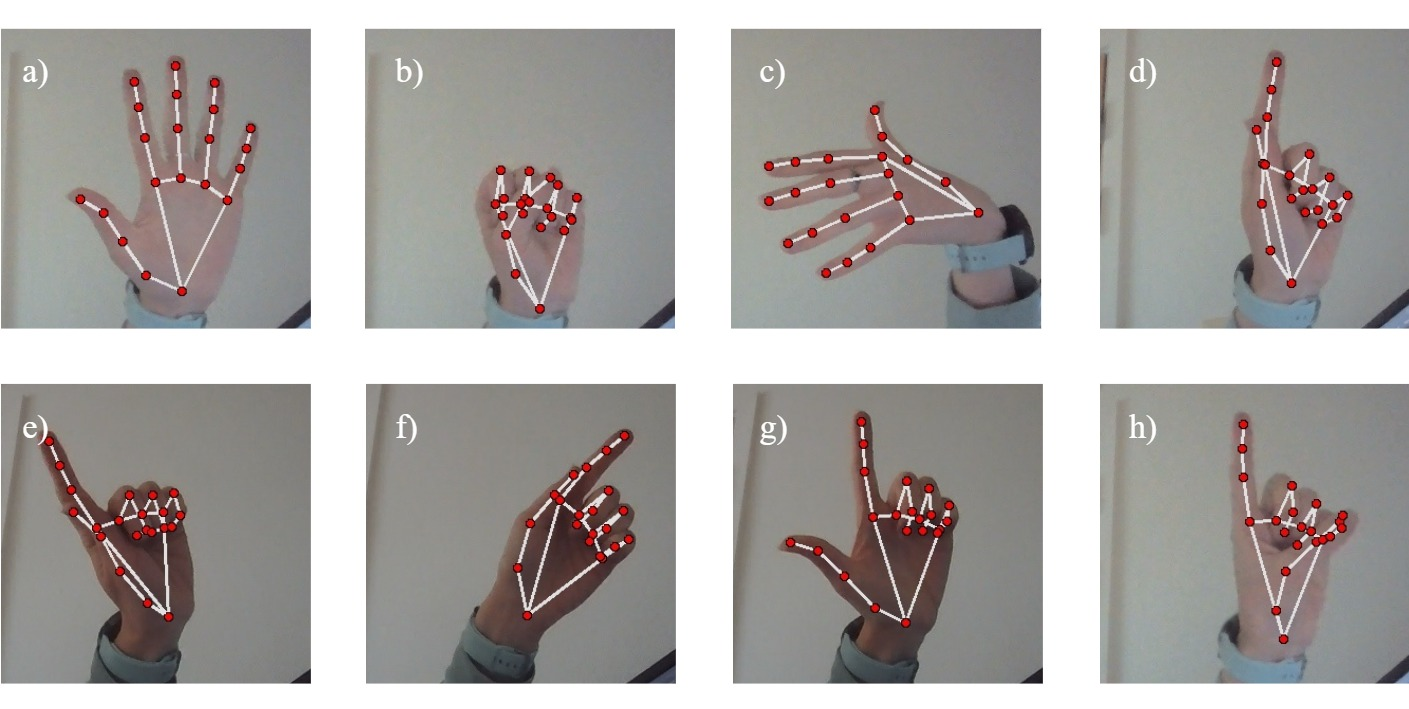
\includegraphics[width=\textwidth, keepaspectratio]{img/hand-gestures.jpg}
  \caption{Gestures detected by the program to control the drone's movement. a) Open hand, b) fist, c) backhand, d) index point up, e) index point left, f) index point right, g) thumb point left, h) thumb point right}
  \label{fig:hand-gestures}
\end{figure}


The program execution is outlined in figure \ref{fig:hands-loop}.
After all the necessary options have been set, a new thread is started to run the pilot queue loop detailed in \ref{subsec:pilot-module}, which waits for new commands.
On the main thread, the GUI loop runs endlessly until the user quits the program, queuing actions based on gestures calculated from retrieved images and on user input on the keyboard, according to the mapping defined in the \texttt{input} module\footnote{\url{https://github.com/l-gonz/tfg-giaa-dronecontrol/blob/main/dronecontrol/common/input.py}}.

\begin{figure}
  \centering
  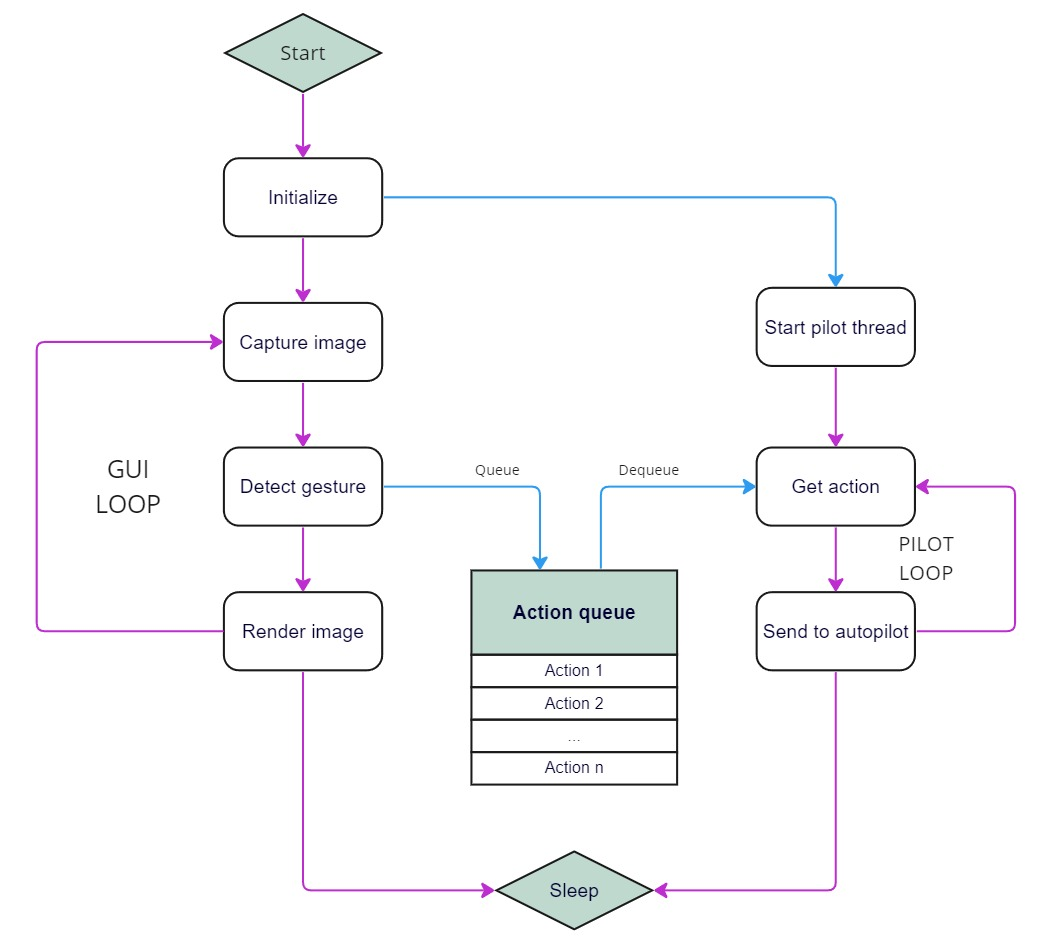
\includegraphics[width=0.8\textwidth, keepaspectratio]{img/hand-loop.jpg}
  \caption{Execution flow for the running loop in the hand-gesture control solution.}
  \label{fig:hands-loop}
\end{figure}

 
\section{Final solution: human following}
\label{sec:follow}

The intention behind developing a UAV control solution that implements tracking and following of humans is to show how the PX4 open-source development platform and its related projects, MAVLink and MAVSDK, can be used to design complex real-life applications without the need for expensive state-of-the-art proprietary hardware.
The only requirements of the follow application are a PX4-enabled flight controller installed in an aerial vehicle, a companion computer of appropriate dimensions that can be mounted on board the vehicle and any camera that can be connected to the companion computer via USB.
During the program execution, the drone can be controlled via an RC controller, an external ground station application or keyboard input directly to the companion computer through, for example, a secure shell using the SSH protocol.

For safety, the follow mechanism only engages when the flight mode on the vehicle is changed to offboard mode, for example, by activating a configured switch in the RC controller, and stops automatically if the connection to the computer is lost or any of the configured fail-safes are triggered, like low battery, loss of RC or GPS signal or vehicle attitude exceeding a predefined pitch and roll value for longer than a specified time.
In this mode, the vehicle will attempt to find a single person in its field of view and follow their movements by changing its yaw and forward velocity to match horizontal movements and distance changes, respectively.

\begin{figure}
  \centering
  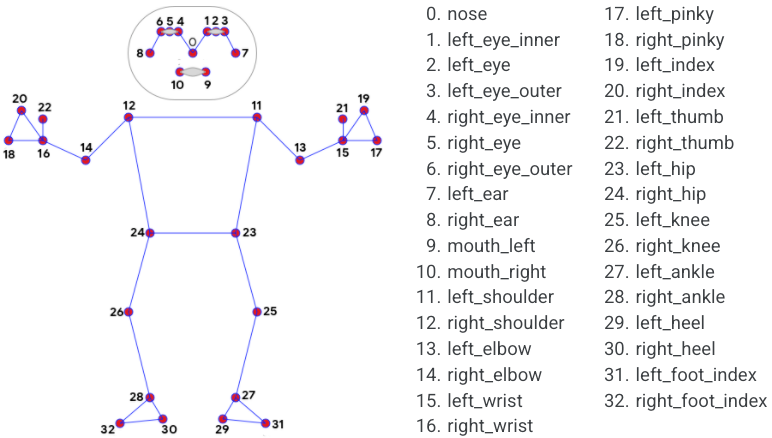
\includegraphics[width=\textwidth, keepaspectratio]{img/pose-landmarks.png}
  \caption{Landmarks extracted from detected human figures by the MediaPipe Pose solution}
  \source{Adapted from \citetitle{mp-pose} \cite{mp-pose}}
  \label{fig:pose-landmarks}
\end{figure}

During the program execution and while the offboard mode and the follow mechanism are engaged, the system continuously retrieves images from the offboard camera that are fed into the MediaPipe Pose \cite{mp-pose-paper} computer vision library to extract pose landmarks from it in the form of 2D coordinates.
Figure \ref{fig:pose-landmarks} shows the features extracted by the algorithm and their correspondence to the human body.
These coordinates are used to draw a bounding rectangle around the detected person and to validate that the received landmarks match the general pose of a person standing up.
Figure \ref{fig:pose-validation} shows some examples of the validation checks running on the raw landmarks extracted from an image.
To prevent unwanted movements, the vehicle will always stop and hover whenever it becomes impossible to detect a person in the image received or its features do not match the expected geometry.
After a valid bounding box has been defined around the target person, its position with respect to the camera's field of view is sent to a control mechanism composed of two independent PID controllers. The theory behind these controllers is explained in section \ref{subsec:pid-tools}.

\begin{figure}
  \centering
  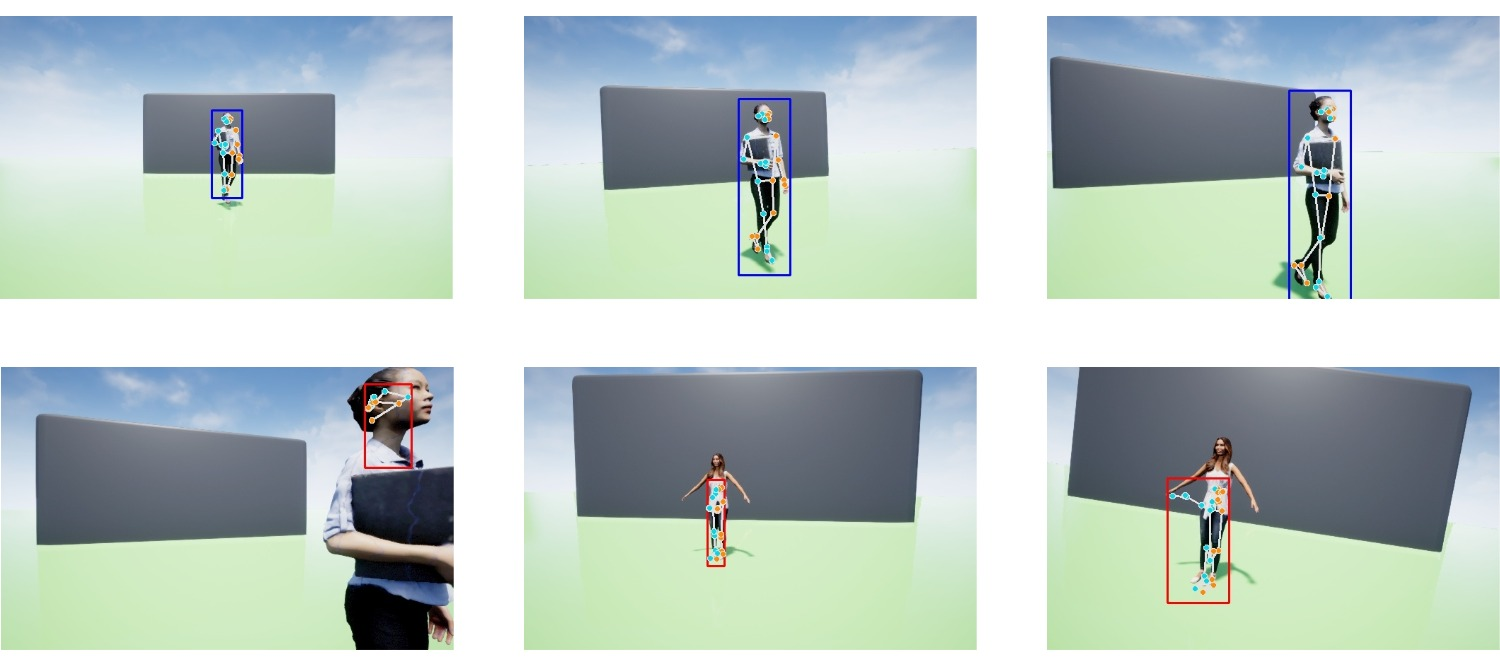
\includegraphics[width=\textwidth, keepaspectratio]{img/pose-validation.jpg}
  \caption{Valid versus invalid poses detected by the follow solution}
  \label{fig:pose-validation}
\end{figure}

The first of the PID controllers is in charge of controlling the yaw velocity of the vehicle to respond to horizontal movements in the x direction of the image.
It takes as input the x coordinate of the centre point of the bounding box, and its target is the middle point of the screen.
Therefore, this controller will output velocity commands to maintain the bounding box centred horizontally in its field of view.
The second PID controller controls the forward velocity of the vehicle to respond to distance changes of the person getting closer or farther away from the drone.
It takes as input the height of the calculated bounding box as a percentage of the total height of the image and works to keep it within a value that matches the desired distance to maintain between the person and the vehicle by moving forwards when the height is too low and backwards when it is too high.
The exact percentage of the image height covered by an average person at a given distance depends on the camera used, so the target height of the controller needs to be set through trial and error for each separate video source.
Figure \ref{fig:follow-input-calcs} shows how these two inputs are extracted from the coordinates of the bounding box detected around the figure.

\begin{figure}
  \centering
  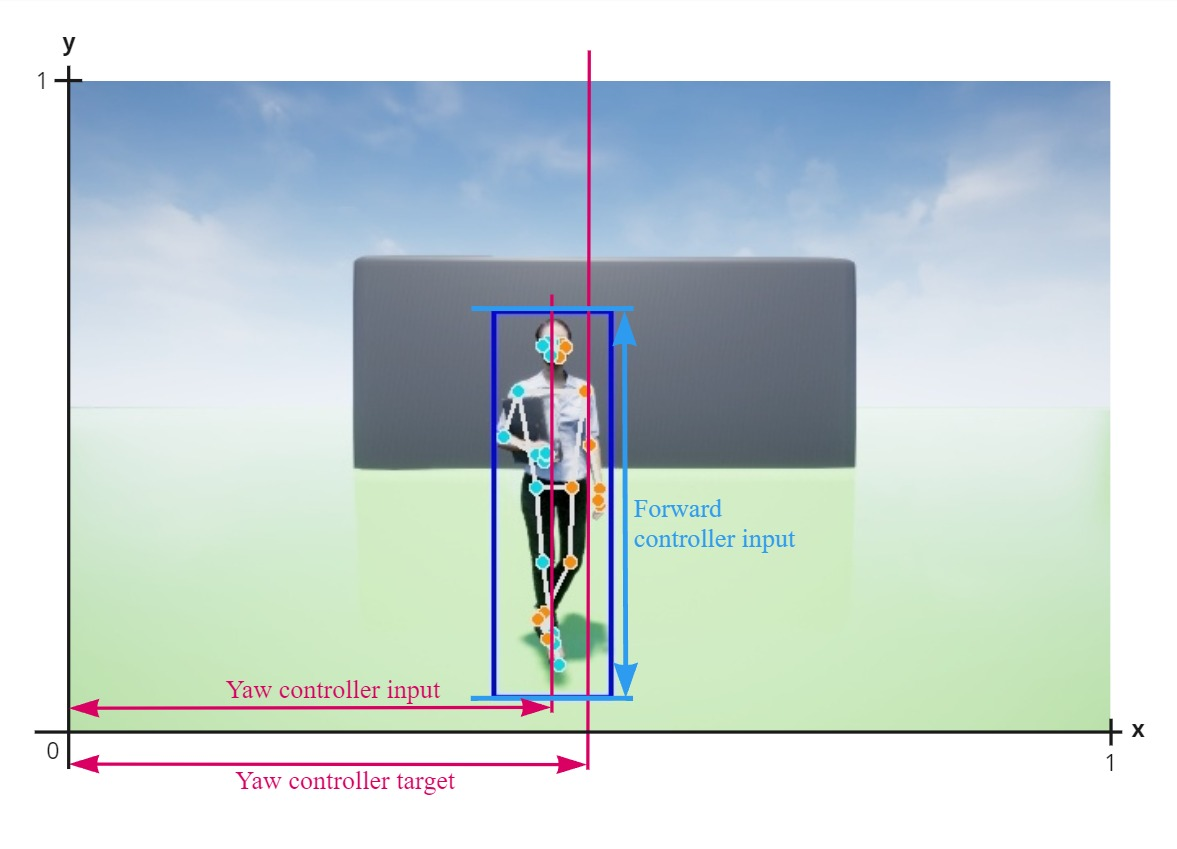
\includegraphics[width=\textwidth, keepaspectratio]{img/pose-calculations.jpg}
  \caption{Calculation of horizontal position and height of figure from the detected bounding box.}
  \label{fig:follow-input-calcs}
\end{figure}


A diagram summarizing the structure of the follow module\footnote{\url{https://github.com/l-gonz/tfg-giaa-dronecontrol/blob/main/dronecontrol/follow/follow.py}} can be seen in figure \ref{fig:follow-loop}.
After connecting to the pilot module with the starting options provided, the main loop runs continuously until the user quits the program.
For each iteration, a new image is retrieved, pose features are extracted from it, and a bounding box is calculated.
Then, and only if the vehicle is in offboard flight mode, the calculated positions will be fed into the PID controller to get a velocity output to send to the pilot.
Keyboard control is also available to send manual commands to the vehicle directly.

\begin{figure}
  \centering
  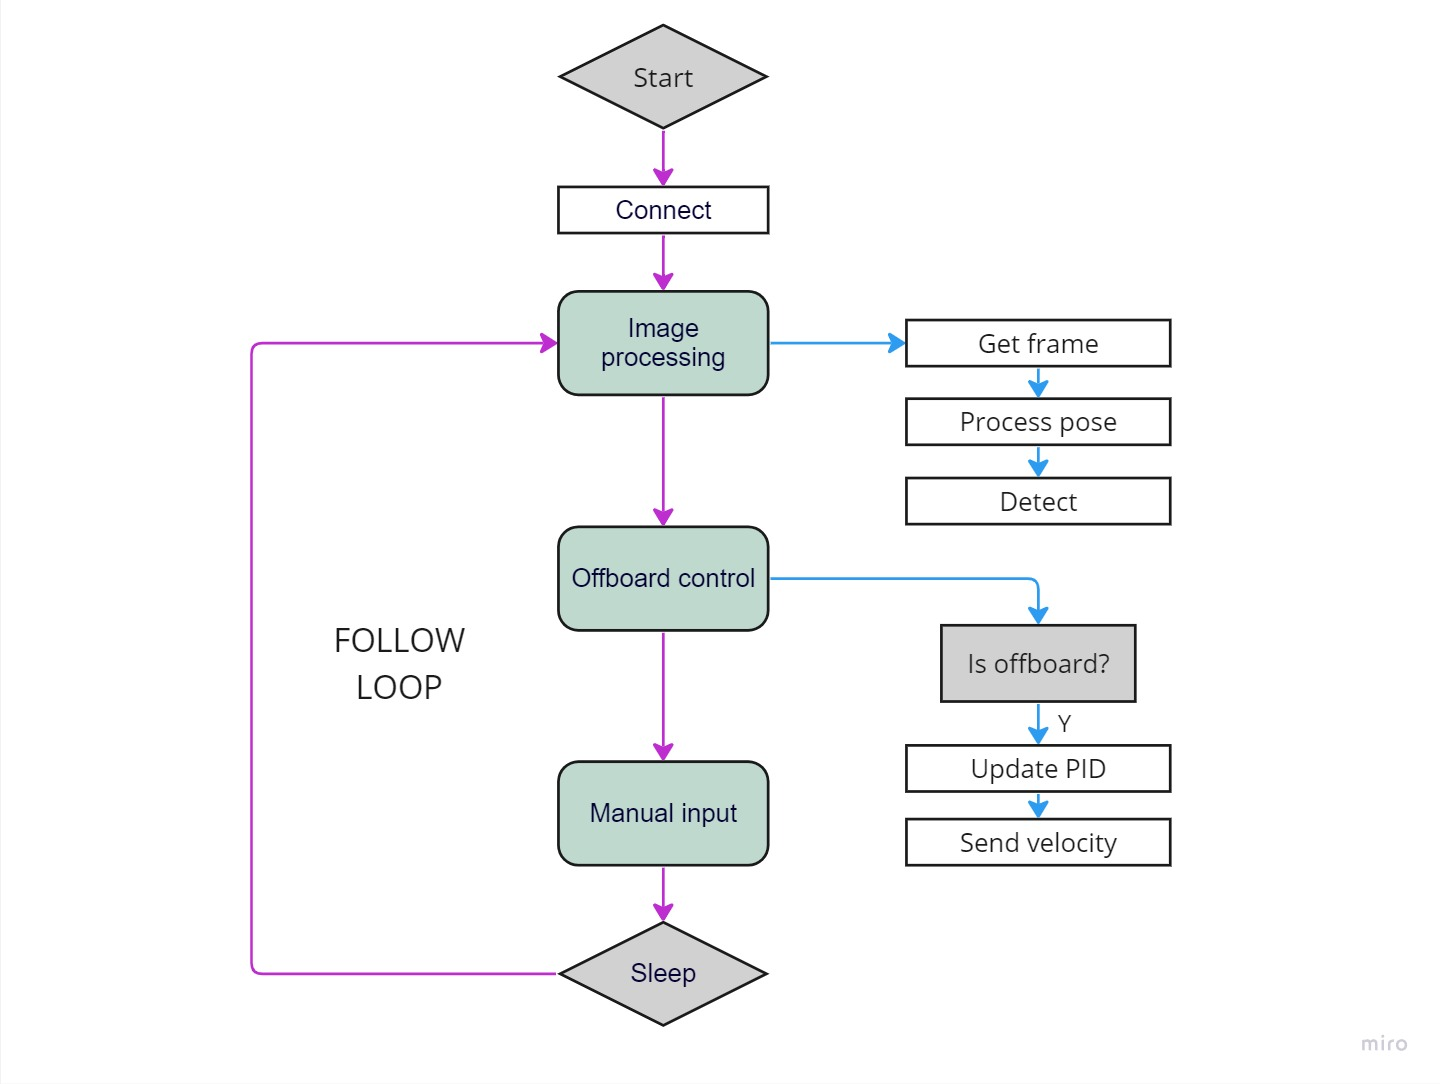
\includegraphics[width=0.9\textwidth, keepaspectratio]{img/follow-loop.jpg}
  \caption{Execution flow for the running loop in the follow control solution}
  \label{fig:follow-loop}
\end{figure}




\subsection{PID tools}
\label{subsec:pid-tools}

Two additional utilities have been developed for tuning and measuring the performance of the PID controllers.
These tools are used in section \ref{sec:test-1-pid} to set the correct values in the controller coefficients empirically.
A proportional-integral-derivative (PID) is a control loop mechanism commonly used in systems requiring continuously modulated control.
It works by continuously calculating an error value from the difference between the received input on a chosen process variable, which in this case is the detected position of a person in the frame, and the desired set point for that variable, a position centred in the frame.
From the error value, the output for the controller is calculated according to this equation:

\begin{equation}
    u(t)= K_p e(t) + K_i \int{e(t)dt} + K_d \frac{de(t)}{dt}
    \label{eq:pid}
\end{equation}
\begin{conditions}
u(t)  &   PID control variable \\
K_p   &   proportional gain \\
K_i   &   integral gain \\
K_d   &   derivative gain \\
e(t)  &   error value \\
de    &   change in error value \\
dt    &   change in time
\end{conditions}

The PID controllers in this project employ the freely-available \texttt{simple-pid} library for Python \cite{pid-library}, which provides all the necessary error calculations already implemented.
It is only necessary to provide the coefficients, or tunings, and the set point for the controller and then call it periodically with an updated input value to receive the output.
In the Dronecontrol application, it is the \texttt{controller} module\footnote{\url{https://github.com/l-gonz/tfg-giaa-dronecontrol/blob/main/dronecontrol/follow/controller.py}} the one that interacts with the \texttt{simple-pid} library to feed and receive the correct values to the PID controllers calculated from the bounding box around the detected person.

Since the most straightforward way to decide the coefficients for a controller is to test different combinations empirically, a small \texttt{tune\_controller} tool has been developed to help with the process\footnote{\url{https://github.com/l-gonz/tfg-giaa-dronecontrol/blob/main/dronecontrol/tools/tune_controller.py}}.
With it, it is possible to specify a range of potential coefficients and test the response of the system on the images retrieved from AirSim and a simulated flight controller (either SITL or HITL can be used).
For each value to be checked, the simulated person to be followed starts in an offset position from the target centre.
Then, the controller is engaged with the test values, and its detected position input and calculated velocity output a plotted in a graph for analysis.
Finally, the vehicle returns to the starting position to reset the environment for the next value to be checked.
The tool is run with the following command: \mintinline{bash}{dronecontrol tools tune}, and can be started with the option \texttt{--yaw} or \texttt{--forward} to decide which specific controller should be tuned.
The other one is deactivated during the test to visualize the effect of the examined values more easily.
Each coefficient can be tested separately by providing fixed values to the other two parameters.

The second tool (\texttt{test\_controller}\footnote{\url{https://github.com/l-gonz/tfg-giaa-dronecontrol/blob/main/dronecontrol/tools/test_controller.py}}) is designed to check the controllers' performance and works slightly differently from the previous one.
The underlying process is the same: engage the controller in an offset position and wait until the movement has stopped before resetting and running again.
However, this tool aims to display how an already-tuned controller reacts to different position inputs for the camera.
This way, the parameter coefficients remain the same for the entire test while the relative position between the vehicle and the person followed varies.
During the execution, both the yaw and the forward controller are activated simultaneously to obtain results closer to what will be expected during actual flight.
However, the test tool can be run in either yaw or forward mode so that the distances to be tested between the vehicle and the person vary either left to right or forward to backward, respectively.
The objective is to measure how the vehicle will react to increasingly bigger differences to the target position to ensure that the movement is stable and that safety is maintained during the entire flight.
A complete execution of this tool for both modes is shown in section \ref{subsec:pid-test-controller}.


\subsection{Safety mechanisms}
\label{subsec:safety}

The Dronecontrol application implements a very experimental vision-based guidance system.
Therefore, to carry out flight tests with real-life conditions, it is necessary to ensure that both the software implements sufficient safety mechanisms to prevent accidents.
Some of these defences employed are part of the developed code, and others are activated simply from the PX4 safety configuration.

In the first place, the Dronecontrol computer vision module prevents accepting as valid input objects that may have been detected wrongly as a person by the MediaPipe algorithm.
This is determined by accepting only received feature points that have a minimum resemblance to a standing human figure, where the bounding box's height is always greater than its width and with the features associated with head, shoulder, hip, knee and ankle stacked from top to bottom in that order.
If any of these checks fail, or if there is no detection output at all received from the library for the current frame, the vehicle will go into Hold flight mode, discarding queued velocity commands, if any, and making the drone hover over its current position.
These checks are implemented in the \texttt{image\_processing} module\footnote{\url{https://github.com/l-gonz/tfg-giaa-dronecontrol/blob/main/dronecontrol/follow/image_processing.py}} for the follow solution.

The second safety mechanism relates to the PID controllers and the pilot module and works by limiting the maximum possible velocity of the vehicle at all points during the execution.
This is done both inside the Dronecontrol application by setting up output limits on the PID controllers that prevent the guidance system from sending abnormal velocity commands to the flight controller, and from the PX4 autopilot itself as a fallback in case of issues with the custom MAVLink integration or the companion computer as a whole, by setting the \texttt{MPC\_XY\_VEL\_ALL} parameter in the autopilot configuration which limits the overall horizontal velocity of the vehicle.

Other safety configuration options included as part of the PX4 autopilot detect undesired behaviour in the flight conditions and trigger a flight mode change to either Hold (hover) or Return (fly back to takeoff position and land), as documented in \citetitle{px4-docs-safety} \cite{px4-docs-safety}.
Some of the detected failure conditions are:
\begin{enumerate}
    \item Lost connection to companion computer while in Offboard mode.
    \item RC transmitter link lost while in manual modes, which can be extended to trigger in Offboard mode.
    \item Lost GPS position, when the quality of the PX4 position estimate falls below acceptable levels.
    \item Low battery during flight.
    \item Vehicle unexpectedly flips.
\end{enumerate}

The last safety mechanism to mention is not based on automatic detection by the developed software or the autopilot but on active surveillance of the system's behaviour during flight by the operator in control of the vehicle.
With an RC controller configured with a switch to control flight mode, it is possible to deactivate Offboard mode at any moment, which will make the vehicle disregard all instructions from the companion computer and assume complete control of the vehicle either through a GPS-assisted mode or fully manual flight.
A secondary switch in the RC controller can be configured as a kill switch for a last-resort option to stop all motor outputs immediately.
This possibility is most useful when the vehicle is on the ground and cannot manage to take off upwards since there is a danger of breaking the propellers against the ground.
